\documentclass[12pt]{article}
%\usepackage{polski}
\usepackage{makecell}
\usepackage[colorlinks=true,citecolor=blue,linkcolor=blue, urlcolor=blue]{hyperref}
\usepackage{graphicx}
\usepackage[ruled]{algorithm2e}
\usepackage{algpseudocode}
\usepackage{amsmath}
\usepackage{caption}
\setlength\parindent{0pt}
\begin{document}

    \title{Reproduction of SNOW paper \\ \vspace{5mm} \large Deep Learning with Multiple Tasks 2020/2021}
    \author{Wiktor Daniec, Paweł Goliszewski, Konrad Wójtowicz}
    \date{}
    \maketitle


    \section{Introduction}

    Creating models which will be able to handle multiple tasks is current object of research in machine learning field.
    People usually do not need thousands of examples (like many ML model do) to learn how to classify objects into some number of classes of object - they usually use information learned through entire life and adapt quickly to new tasks.
    Idea is to use 'knowledge' from model trained on the other task to learn faster how to manage other task.
    Authors of paper \cite{paper} tackle the problem of image classification.
    They use pretrained model with smaller model connected to it to perform classification task on other classes.
    Our goal was to try to reproduce their results.


    \section{SNOW model architecture}

    This model uses 2 models connected via operation called Channel Pooling which will be described later.
    One model (called source model) is ResNet50 pretrained on ImageNet dataset with frozen weights.
    It is connected after each convolutional layer with second model (called delta model) which is smaller version of Resnet (in our experiments channels reduced by 8) with randomly initialized and trainable weights.
    We put image tensor to both model inputs, and we use only the output of the delta model into consideration.

    \begin{figure}
        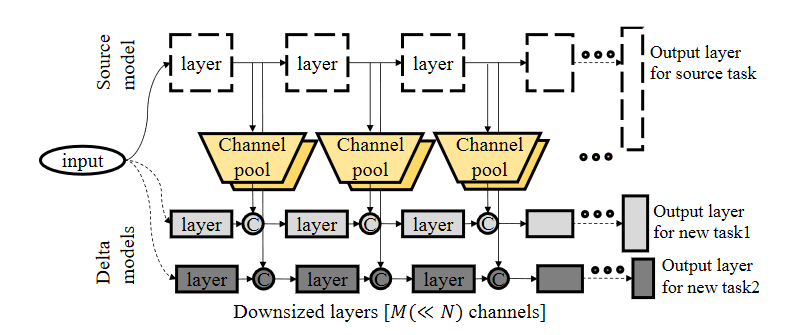
\includegraphics{SNOW.png}
        \caption{Illustration of SNOW model}
    \end{figure}

    \subsection{Channel pooling operation}

    Channel pooling (CP) operation behaves differently during training stage and the evaluation stage.

    CP layer contains weight vector $w$ of size $N$ where $N$ is also number of input tensor layers.
    If it is training time we sample vector size $N$ from normal distribution of mean 0 and standard deviation $\sigma$, and add it to the weights vector obtaining $rand_v$ vector.
    We take indexes of the $L$ biggest values of $rand_v$.
    We take $L$ channels of the input given by those indexes multiplied by $w$ element-wisely.
    We concatenate the result to the corresponding input int the delta model.

    \begin{algorithm}
        $w$: channel pooling weight ($N\times1$ vector)\;
        $x$: input tensor (with $N$ channels)\;
        \SetKwFunction{FMain}{ChannelPoolingFroward}
        \SetKwProg{Pn}{Function}{:}{\KwRet x}
        \Pn{\FMain{$x$}}{
            \eIf{training}{
                $rand_v=w+\mathcal{N}(0,\sigma)$\;
                $\_,idx=\text{topK}(rand_v,L)$\;
                $selected\_weights=w[idx]$
            }{
                $selected\_weights,idx=\text{topK}(rand_v,L)$\;
            }
            \EndIf
            $x = x[idx]$\;
            $x = x \bigotimes selected\_weights$\;
        }
        \caption{Channel Pooling pseudocode}\label{alg:algorithm}
    \end{algorithm}


    \section{Transfer learning}

    We use some standard transfer learning techniques for comparison.
    Those techniques are:
    \begin{itemize}
        \item full fine-tuning (FT) - We use pretrained ResNet50, and we modify last layer to adjust number of classes to a new task. Then we train network with all trainable parameters on a new task.
        \item feature extraction (FE) - Similarly as above, but weights of first 3 bottlenecks are frozen.
        \item final layer only (FO) - Similarly as above, but only last linear layer is not frozen.
    \end{itemize}


    \section{Experiments}

    \subsection{Datasets}

    We used 5 datasets: Action, Cars, DTD, Birds, Food-101.

    Action dataset contains 9532 images (4000 in training dataset and 5532 in the test dataset) divided into 40 classes.
    The images are photos of people performing an action, for instance: jumping, fixing a car, playing guitar etc.

    Cars dataset contains 196 categories of car of 16185 images in total (8144 in training dataset and 8041 in the test dataset)
    They are photos of different models of cars like: 2012 Tesla Model S, 2012 BMW M3 coupe, etc.

    There are 47 categories in DTD (Describable Textures Dataset) and 5640 images (3760 in training dataset and 1880 in the test dataset).
    Images contains different textures, for example: grid pattern, stripped pattern etc.

    Birds dataset is made of 8891 photos (5994 in training set and 2897 in test dataset) of 200 species of birds.

    Food-101 dataset contains 11000 photographs of 101 categories of meals like: hot dog, risotto etc.
    There are 75750 images in train dataset and 25250 ones in the test dataset.
    Unfortunately we do not have results of training on this dataset because of lack of time and computational resources.

    For each dataset we perform normalization and resize to $224\times224$.

    \subsection{Transfer learning}

    On~\ref{fig:valacc_tl} we present validation accuracy during training of three TL methods mentioned earlier.
    \begin{figure}
        \centering
        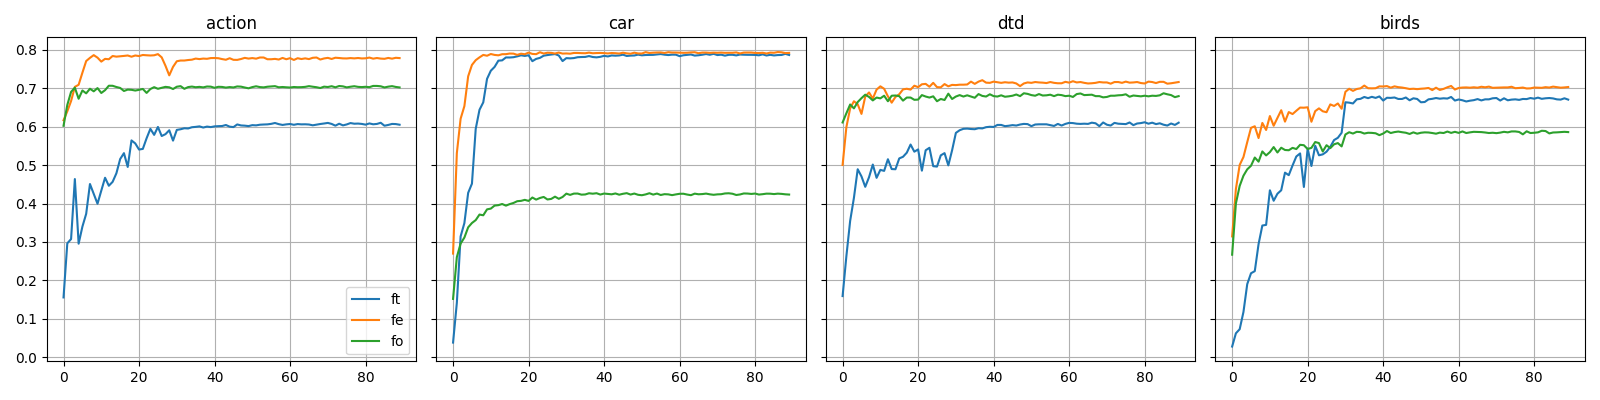
\includegraphics[width=\linewidth]{valacc}
        \caption{Accuracy at test set of Transfer learning methods}
        \label{fig:valacc_tl}
    \end{figure}

    \subsection{SNOW}

    We performed experiments on all datasets using SNOW model.
    Hyperparameters' values are in table \ref{tab:1}.
    $K$ is parameter which means how many times delta model is smaller (by number of channels).
    We take $\frac{1}{M}$ of input channels as a parameter $L$ of channel pooling layer.
    We use stochastic gradient descent algorithm with momentum and weight decay.
    We also use step learning rate scheduler which multiplies learning rate by $0.1$ every $10$ epochs.

    \begin{table}
        \centering
        \begin{tabular}{|c|c|c|c|c|c|c|c|c|}
            \hline
            \thead{Parameter} & \thead{$K$} & \thead{$M$} & \thead{$\sigma^2$} & \thead{batch \\size} & \thead{initial \\learning \\rate} & \thead{momentum} & \thead{weight \\decay} & \thead{training \\epochs} \\
            \hline
            Value & $8$ & $8$ & $0.001$ & $64$ & $1.0$ & $0.9$ & $0.0001$ & $50$ \\
            \hline
        \end{tabular}
        \caption{SNOW model hyperparameters}
        \label{tab:1}
    \end{table}

    \begin{table}
        \centering
        \begin{tabular}{|c|c|c|c|c|}
            \hline
            \thead{Dataset}          & \thead{Action} & \thead{Cars} & \thead{DTD} & \thead{Birds} \\
            \hline
            Max accuracy on test set & $10.59\%$      & $12.70\%$    & $30.53\%$   & $1.38\%$      \\
            \hline
        \end{tabular}
        \caption{SNOW results (last running)}
        \label{tab:2}
    \end{table}

    \begin{figure}
        \centering
        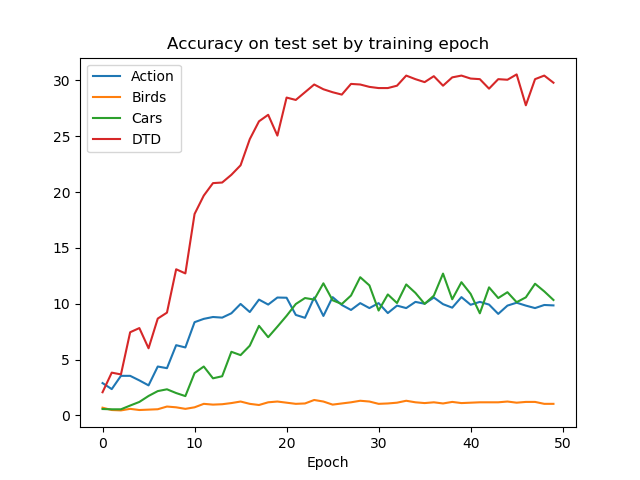
\includegraphics[width=\linewidth]{accs}
        \caption{Plot of accuracy by epoch (last running)}
        \label{fig:accs}
    \end{figure}


    \begin{figure}
        \centering
        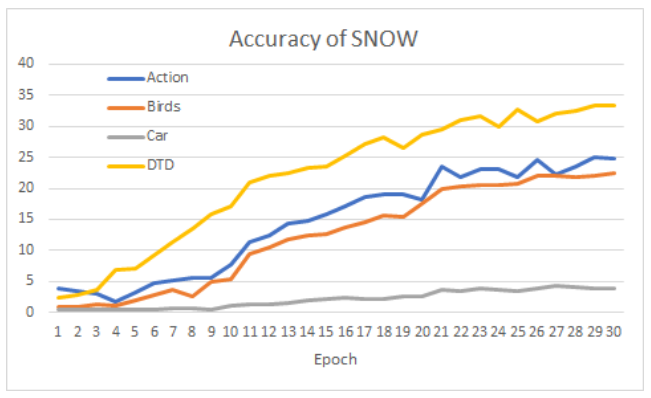
\includegraphics[width=\linewidth]{accs_old}
        \caption{Plot of accuracy by epoch (from former run)}
        \label{fig:accs2}
    \end{figure}

    As we see from the plots: \ref{fig:accs} and \ref{fig:accs2} during different runs training stuck in different local minima.
    This differs from what was shown in \cite{paper}.
    Models, we have implemented, were not learning so quickly and could not reach accuracies those obtained by transfer learning techniques.
    The reason of that can be differences between our implementation and what authors have coded.
    Maybe Channel Pooling operation is placed too densely in the model - we suppose that injection of results of frozen weights of source model may perform poor if it is used in every convolutional layer.

    \subsection{Evaluation and Throughput}

    \begin{table}
        \centering
        \begin{tabular}{|c|c|c|c|c|}
            \hline
            \thead{Dataset} & \thead{Action} & \thead{Cars} & \thead{DTD} & \thead{Birds} \\
            \hline
            SNOW            & $217.09$       & $62.86$      & $214.04$    & $218.89$      \\
            \hline
        \end{tabular}
        \caption{Throughput (images per second)}
        \label{tab:3}
    \end{table}

    We see that result from cars dataset is much lower than others.
    It can be caused by bigger size of those images.
    We can not compare results with those from paper because we use different computation server and graphics cards.
    We used Nvidia RTX2080Ti and RTX1080 GPUs. Each has memory of 11GB RAM what forced us to decrease batch size to 64.

    \subsection{Visualization of filters}

    We have done visualization of $3x7x7$ filters of models trained on each of the datasets.
    Plots (\ref{fig:filters_action}, \ref{fig:filters_birds}, \ref{fig:filters_cars} and \ref{fig:filters_dtd}) contain delta model's filters of initial convolutional layer in the first row and source model's ones (eight of highest weigght in channel pooling layer).

    We see that the source model's filters vary more than those from the delta models.
    This could mean filters in well-trained model are more specialized.

    \begin{figure}
        \centering
        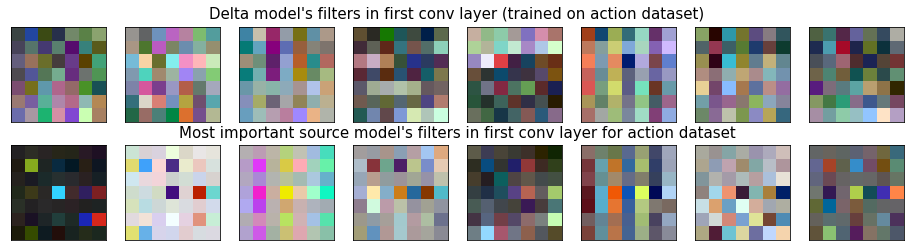
\includegraphics[width=\linewidth]{action}
        \caption{Visualisation of filters trained on Action dataset}
        \label{fig:filters_action}
    \end{figure}


    \begin{figure}
        \centering
        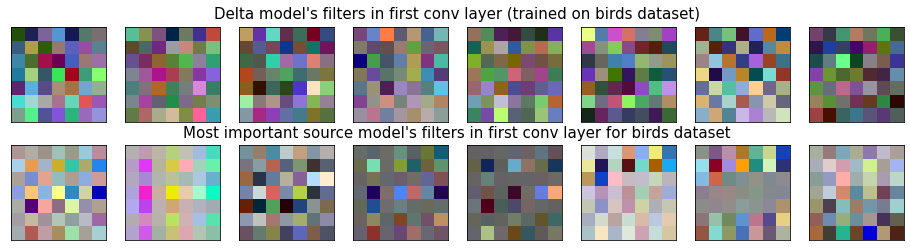
\includegraphics[width=\linewidth]{birds}
        \caption{Visualisation of filters trained on Birds dataset}
        \label{fig:filters_birds}
    \end{figure}

    \begin{figure}
        \centering
        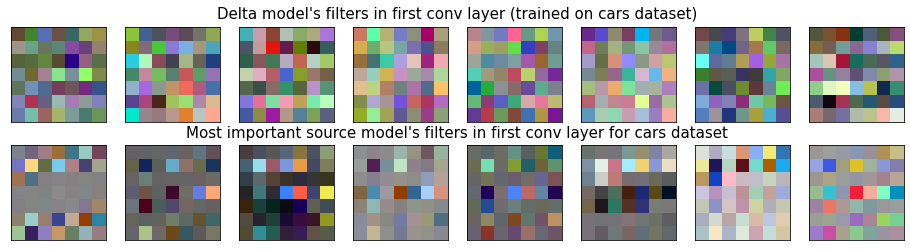
\includegraphics[width=\linewidth]{cars}
        \caption{Visualisation of filters trained on Action dataset}
        \label{fig:filters_cars}
    \end{figure}

    \begin{figure}
        \centering
        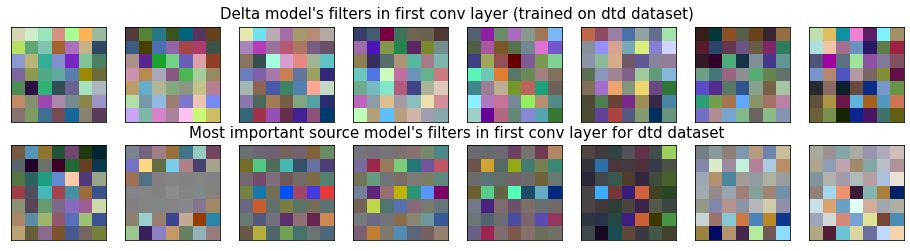
\includegraphics[width=\linewidth]{dtd}
        \caption{Visualisation of filters trained on DTD dataset}
        \label{fig:filters_dtd}
    \end{figure}

    \section{Conslusions}

    Unfortunately we did not manage to reproduce results of authors of \cite{paper}.
    Probably it was a hard task because of no code published by authors and lack of the details in paper.
    It was hard to decide how densely channel pooling operation should be placed.
    We placed it after each convolutional layer in the model.
    We have sent emails to the authors to get more details, but we have not got any responses.
    The SNOW approach did not learn as quickly as transfer learning approaches, but it is still faster than learning from scratch.
    We did not manage to perform training on Food-101 dataset because of technical issues (we were unable to parallelize dataloader because of weird exception) and lack of time.
    The computational machine which belong to Robotics and Artificial Intelligence Students' Association of Jagiellonian University was not so fast as one used by authors of the paper.

    \begin{figure}
        \centering
        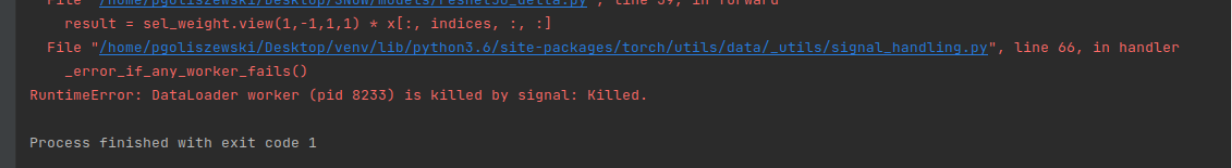
\includegraphics[width=\linewidth]{exception}
        \caption{Exception which was showing up randomly after several epochs of training with paraller data loaders}
        \label{fig:exception}
    \end{figure}


    \begin{thebibliography}{99}
        \bibitem{paper} \href{https://openreview.net/pdf?id=rJxtgJBKDr}{https://openreview.net/pdf?id=rJxtgJBKDr} \\
        Chungkuk Yoo, Bumsoo Kang, Minsik Cho, SNOW: Subscribing to Knowledge via Channel Pooling for Transfer \& Lifelong Learning of Convolutional Neural Networks, ICLR 2020
    \end{thebibliography}
\end{document}
